% ============================================================
%  Metoda Kompjuterike në Aktuaristikë — Template Beamer (Singapore)
%  FIMIF · UPT  |  Assoc. Prof. Endri Raço, PhD
%  Kompilim: pdflatex (2 herë, për navigimin Singapore)
%  Logo: vendos logo_upt.png dhe logo_fimif.png në të njëjtën dosje.
%        Nëse mungojnë, shfaqet një vend-mbajtës i thjeshtë.
% ============================================================
\documentclass[aspectratio=169,10pt,xcolor={dvipsnames,table}]{beamer}

% ---------- Tema ----------
\usetheme{Singapore}
\setbeamertemplate{navigation symbols}{}
\setbeamertemplate{footline}[frame number]

% ---------- Ngjyrat (blu UPT + ngjyra theksi) ----------
\definecolor{uptblue}{HTML}{1E325A}
\definecolor{uptmid}{HTML}{2C5AA0}
\definecolor{uptlight}{HTML}{E8EEF7}
\definecolor{accent}{HTML}{D97706}
\definecolor{okgreen}{HTML}{15803D}
\definecolor{warnred}{HTML}{B91C1C}
\definecolor{codebg}{HTML}{F6F8FA}

\setbeamercolor{palette primary}{bg=uptblue,fg=white}
\setbeamercolor{palette secondary}{bg=uptmid,fg=white}
\setbeamercolor{palette tertiary}{bg=uptblue,fg=white}
\setbeamercolor{section in head/foot}{bg=uptlight,fg=uptblue}
\setbeamercolor{frametitle}{fg=uptblue,bg=white}
\setbeamercolor{title}{fg=uptblue}
\setbeamercolor{structure}{fg=uptmid}
\setbeamercolor{item}{fg=accent}
\setbeamercolor{block title}{bg=uptmid,fg=white}
\setbeamercolor{block body}{bg=uptlight}
\setbeamerfont{frametitle}{series=\bfseries,size=\large}

% ---------- Paketat ----------
\usepackage[utf8]{inputenc}
\usepackage[T1]{fontenc}
\usepackage{lmodern}
\usepackage{amsmath,amssymb,bm}
\usepackage{booktabs}
\usepackage{graphicx}
\usepackage{tikz}
\usetikzlibrary{positioning,arrows.meta,shapes.geometric,calc,trees}
\usepackage{pgfplots}
\pgfplotsset{compat=1.18}
\usepackage[most]{tcolorbox}
\usepackage{listings}
\usepackage{hyperref}
\hypersetup{colorlinks=true,linkcolor=uptmid,urlcolor=uptmid}

% ---------- Kutitë pedagogjike ----------
\newtcolorbox{Definicion}[1][]{colback=uptlight,colframe=uptblue,fonttitle=\bfseries,title={Definicion #1},boxrule=0.6pt,arc=2pt,left=4pt,right=4pt,top=2pt,bottom=2pt}
\newtcolorbox{Teoreme}[1][]{colback=white,colframe=uptmid,fonttitle=\bfseries,title={Teoremë #1},boxrule=0.6pt,arc=2pt}
\newtcolorbox{Shembull}[1][]{colback=green!4,colframe=okgreen,fonttitle=\bfseries,title={Shembull #1},boxrule=0.6pt,arc=2pt}
\newtcolorbox{Ushtrim}[1][]{colback=orange!5,colframe=accent,fonttitle=\bfseries,title={Radha jote! #1},boxrule=0.6pt,arc=2pt}
\newtcolorbox{Gabim}[1][]{colback=red!4,colframe=warnred,fonttitle=\bfseries,title={Gabim i zakonshëm #1},boxrule=0.6pt,arc=2pt}
\newtcolorbox{Keshille}[1][]{colback=yellow!6,colframe=yellow!50!black,fonttitle=\bfseries,title={Këshillë #1},boxrule=0.6pt,arc=2pt}
\newtcolorbox{Parashiko}[1][]{colback=purple!4,colframe=purple!70!black,fonttitle=\bfseries,title={Parashiko para se ta ekzekutosh #1},boxrule=0.6pt,arc=2pt}

% ---------- Stili i kodit R ----------
\lstdefinestyle{Rstyle}{
  language=R,
  backgroundcolor=\color{codebg},
  basicstyle=\ttfamily\footnotesize,
  keywordstyle=\color{uptmid}\bfseries,
  commentstyle=\color{gray}\itshape,
  stringstyle=\color{okgreen},
  showstringspaces=false,
  frame=single, rulecolor=\color{uptlight},
  breaklines=true, columns=fullflexible,
  numbers=left, numberstyle=\tiny\color{gray}, numbersep=6pt,
  xleftmargin=12pt, framexleftmargin=12pt,
  literate={ë}{{\"e}}1 {Ë}{{\"E}}1 {ç}{{\c c}}1 {Ç}{{\c C}}1 {<-}{{$\leftarrow$}}1
}
\lstset{style=Rstyle}
\lstdefinestyle{Rout}{columns=fixed,keepspaces=true,basicstyle=\ttfamily\footnotesize\color{uptblue},backgroundcolor=\color{white},frame=leftline,rulecolor=\color{accent},numbers=none,xleftmargin=8pt}

% ---------- Komanda ndihmëse ----------
\newcommand{\Rkey}[1]{\texttt{\textcolor{uptmid}{#1}}}
\newcommand{\termi}[2]{\textbf{#1} (\emph{#2})}
\newcommand{\shkoTe}[2]{\hyperlink{#1}{\beamergotobutton{#2}}}
\newcommand{\kthehu}[1]{\hyperlink{#1}{\beamerreturnbutton{Kthehu}}}

% ---------- Logo (vend-mbajtës nëse mungon skedari) ----------
\newcommand{\logoUPT}{%
  \IfFileExists{logo_upt.png}{\includegraphics[height=0.9cm]{logo_upt.png}}{%
  \tikz{\node[draw=uptblue,thick,rounded corners=2pt,minimum width=1.6cm,minimum height=0.8cm,font=\scriptsize\bfseries,text=uptblue]{UPT};}}}
\newcommand{\logoFIMIF}{%
  \IfFileExists{logo_fimif.png}{\includegraphics[height=0.9cm]{logo_fimif.png}}{%
  \tikz{\node[draw=uptmid,thick,rounded corners=2pt,minimum width=1.6cm,minimum height=0.8cm,font=\scriptsize\bfseries,text=uptmid]{FIMIF};}}}

% ---------- Informacioni i leksionit (ndrysho çdo javë) ----------
\newcommand{\javaNr}{8}
\newcommand{\temaJaves}{Modeli Cox i rreziqeve proporcionale}
\title[MKA · Java \javaNr]{Metoda Kompjuterike në Aktuaristikë}
\subtitle{Java \javaNr: \temaJaves}
\author{Assoc. Prof. Endri Raço, PhD}
\institute{Fakulteti i Inxhinierisë Matematike dhe Inxhinierisë Fizike\\Universiteti Politeknik i Tiranës}
\date{Workshop 7-orësh}
\titlegraphic{\logoUPT\hspace{0.6cm}\logoFIMIF}

\begin{document}

% ===================== FAQJA E TITULLIT =====================
\begin{frame}[plain]
  \titlepage
\end{frame}

\begin{frame}{Plani i ditës (7 orë)}
  \tableofcontents
\end{frame}

% ===================== ORA 1 =====================
\section{Motivimi}
\subsection{Problemi real}

\begin{frame}{Pse na duhet ky model?}
  \begin{itemize}
    \item<1-> Një sigurues jete do të dijë \textbf{sa shpejt} anulohen policat.
    \item<2-> Faktorë: mosha, prima, kanali i shitjes.
    \item<3-> Pyetja: si ndikon secili faktor në \emph{rrezikun e çastit}?
  \end{itemize}
  \onslide<4->{\begin{Keshille}Mbaje mend këtë pyetje — do t'i përgjigjemi në Orën 6 me të dhëna.\end{Keshille}}
\end{frame}

\subsection{Objektivat}
\begin{frame}{Objektivat e mësimit}
  Në fund të ditës do të jesh në gjendje:
  \begin{enumerate}
    \item të shpjegosh \termi{funksionin e rrezikut}{hazard function};
    \item të vlerësosh modelin Cox në R me \Rkey{survival::coxph()};
    \item të interpretosh \termi{raportin e rrezikut}{hazard ratio};
    \item të kontrollosh supozimin PH me mbetjet Schoenfeld.
  \end{enumerate}
\end{frame}

% ===================== ORA 2 =====================
\section{Teoria}
\subsection{Përkufizime}

\begin{frame}{Funksioni i rrezikut}
  \begin{Definicion}[(Hazard)]
    \[
      h(t)=\lim_{\Delta t\to 0}\frac{P(t\le T<t+\Delta t\mid T\ge t)}{\Delta t}
    \]
  \end{Definicion}
  \pause
  \begin{itemize}
    \item $T$ = koha deri te ngjarja (vdekje, anulim, dëm).
    \pause
    \item Lexim: ``shpejtësia'' e ngjarjes, duke ditur që deri në $t$ nuk ka ndodhur.
  \end{itemize}
\end{frame}

\begin{frame}{Modeli Cox — hap pas hapi}
  \begin{align*}
    h(t\mid \bm{x}) &= h_0(t)\,\exp(\bm{\beta}^\top\bm{x}) \\
    \onslide<2->{\frac{h(t\mid \bm{x}_1)}{h(t\mid \bm{x}_2)} &= \exp\!\big(\bm{\beta}^\top(\bm{x}_1-\bm{x}_2)\big)}
  \end{align*}
  \onslide<3->{
  \begin{Teoreme}[(Proporcionaliteti)]
    Raporti nuk varet nga $t$ — prandaj ``rreziqe proporcionale''.
  \end{Teoreme}}
  \onslide<4->{
  \begin{Gabim}$e^{\beta}$ është raport \emph{rreziqesh}, jo raport probabilitetesh.\end{Gabim}}
\end{frame}

% ===================== ORA 3 =====================
\section{Laborator R}
\subsection{Nga zero}

\begin{frame}[fragile]{Kodi R: vlerësimi i modelit}
\begin{lstlisting}
library(survival)
set.seed(2026)                    # riprodhueshmëri
d <- read.csv("lapse_policies.csv")
fit <- coxph(Surv(time, lapse) ~ age + premium + channel,
             data = d)
summary(fit)$coefficients[, c("coef","exp(coef)","Pr(>|z|)")]
\end{lstlisting}
\end{frame}

\begin{frame}[fragile]{Çfarë na tregon rezultati?}
\begin{lstlisting}[style=Rout]
                 coef exp(coef)  Pr(>|z|)
age           -0.021     0.979    <0.001
premium        0.004     1.004    <0.001
channelonline  0.412     1.510    <0.001
\end{lstlisting}
  \begin{itemize}
    \item Shitja \emph{online} rrit rrezikun e anulimit me rreth 51\%.
  \end{itemize}
  \footnotesize\textcolor{gray}{(Rezultat ilustrues në template; në leksion shfaqet output-i i ekzekutuar realisht.)}
\end{frame}

\begin{frame}[label=pyetja1]{Parashiko!}
  \begin{Parashiko}
    Nëse \texttt{premium} rritet me 100, sa ndryshon rreziku?\\[2pt]
    \textbf{A)} +0.4\% \quad \textbf{B)} +49\% \quad \textbf{C)} +4\%
  \end{Parashiko}
  \shkoTe{zgjidhja1}{Shiko zgjidhjen}
\end{frame}

% ===================== ORA 4 =====================
\section{Ilustrime}
\subsection{Grafika}

\begin{frame}{Kurba e mbijetesës (TikZ / pgfplots)}
  \centering
  \begin{tikzpicture}
    \begin{axis}[width=0.75\textwidth,height=0.55\textheight,
      xlabel={Viti i policës $t$},ylabel={$S(t)$},ymin=0,ymax=1.05,
      grid=major,grid style={gray!20},legend pos=north east,
      legend style={font=\footnotesize}]
      \addplot[uptmid,very thick,domain=0:10,samples=100]{exp(-0.10*x)};
      \addplot[accent,very thick,dashed,domain=0:10,samples=100]{exp(-0.10*1.51*x)};
      \legend{Agjent, Online ($HR=1.51$)}
    \end{axis}
  \end{tikzpicture}
\end{frame}

\begin{frame}{Pema binomiale Cox--Ross--Rubinstein (TikZ)}
  \centering
  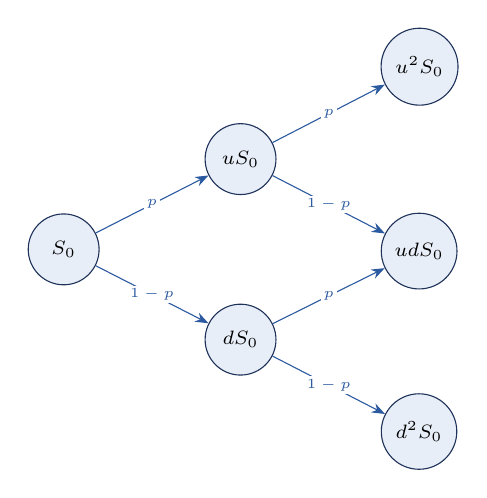
\begin{tikzpicture}[>=Stealth,node distance=1.6cm,
      nd/.style={circle,draw=uptblue,fill=uptlight,minimum size=9mm,font=\scriptsize}]
    \node[nd] (s0) {$S_0$};
    \node[nd,above right=0.5cm and 1.6cm of s0] (u) {$uS_0$};
    \node[nd,below right=0.5cm and 1.6cm of s0] (d) {$dS_0$};
    \node[nd,above right=0.5cm and 1.6cm of u] (uu) {$u^2S_0$};
    \node[nd,below right=0.5cm and 1.6cm of u] (ud) {$udS_0$};
    \node[nd,below right=0.5cm and 1.6cm of d] (dd) {$d^2S_0$};
    \foreach \a/\b/\c in {s0/u/p,s0/d/1-p,u/uu/p,u/ud/1-p,d/ud/p,d/dd/1-p}
      \draw[->,uptmid] (\a) -- node[midway,font=\tiny,fill=white,inner sep=1pt]{$\c$} (\b);
  \end{tikzpicture}
  \[ u=e^{\sigma\sqrt{\Delta t}},\quad d=1/u,\quad p=\frac{e^{r\Delta t}-d}{u-d} \]
\end{frame}

% ===================== ORA 5–6 =====================
\section{Rast studimi}
\subsection{Projekt mini}
\begin{frame}{Rast studimi: anulimet e policave}
  \begin{columns}[T]
    \column{0.5\textwidth}
      \textbf{Të dhënat}
      \begin{itemize}
        \item 2\,000 polica (sintetike)
        \item kohë, ngjarje, kovariate
      \end{itemize}
    \column{0.5\textwidth}
      \textbf{Detyra}
      \begin{enumerate}
        \item Kaplan--Meier sipas kanalit
        \item Cox me 3 kovariate
        \item Kontrolli i PH
      \end{enumerate}
  \end{columns}
\end{frame}

% ===================== ORA 7 =====================
\section{Përmbledhje}
\subsection{Konsolidim}
\begin{frame}{\textcolor{accent}{$\checkmark$} Checkpoint}
  \begin{enumerate}
    \item Çfarë mat $h(t)$?
    \item Pse quhet ``proporcional''?
    \item Si e kontrollon supozimin PH në R?
  \end{enumerate}
\end{frame}

\begin{frame}{Fletë-kujtese}
  \begin{tabular}{@{}ll@{}}
    \toprule
    Detyra & Funksioni R \\ \midrule
    Objekt mbijetese & \Rkey{Surv(time, event)} \\
    Kaplan--Meier & \Rkey{survfit()} \\
    Modeli Cox & \Rkey{coxph()} \\
    Testi PH & \Rkey{cox.zph()} \\ \bottomrule
  \end{tabular}
\end{frame}

% ===================== SHTOJCA =====================
\appendix
\section*{Zgjidhjet}
\begin{frame}[label=zgjidhja1]{Zgjidhja: Parashiko!}
  $e^{0.004\times100}=e^{0.4}\approx1.49 \Rightarrow$ \textbf{B) +49\%}
  \vfill\kthehu{pyetja1}
\end{frame}

\end{document}
